\chapter{Testování}
\label{sec:Testing}\

V~této kapitole je popsáno testování algoritmu optimalizace rychlosti na dráze,
která je popsaná v~kapitole~\ref{sec:PlatformControl}, a~porovnána s~manuálním
řízením i~řízením bez senzoru.

Pro porovnání potřebujeme spočítat za kolik tiků auto projelo jedno kolo. 
Na to můžeme využít data úhlové rychlosti, která je zobrazena 
na obrázku \ref{fig:Laps}.

\begin{figure}[!h]
    \begin{subfigure}{.5\textwidth}
        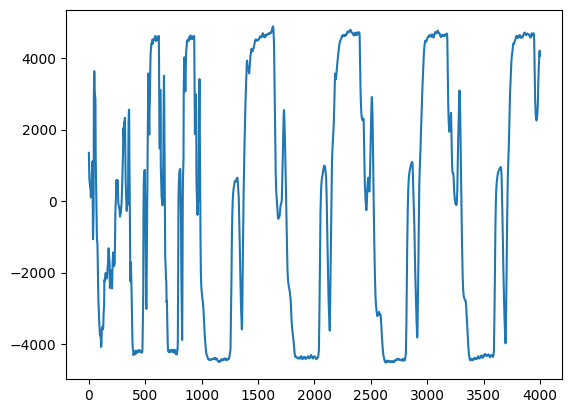
\includegraphics[width = \textwidth]{Figures/LapAuto.png}
        \label{fig:LapsAuto}
        \caption{Automatické řízení se senzory.}
    \end{subfigure}
    \begin{subfigure}{.5\textwidth}
        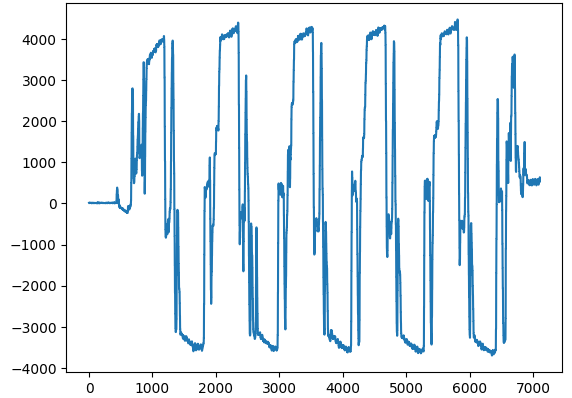
\includegraphics[width = \textwidth]{Figures/LapAutoNoSensors.png}
        \label{fig:LapsAuto}
        \caption{Automatické řízení bez senzorů.}
    \end{subfigure}
    \begin{subfigure}{.5\textwidth}
        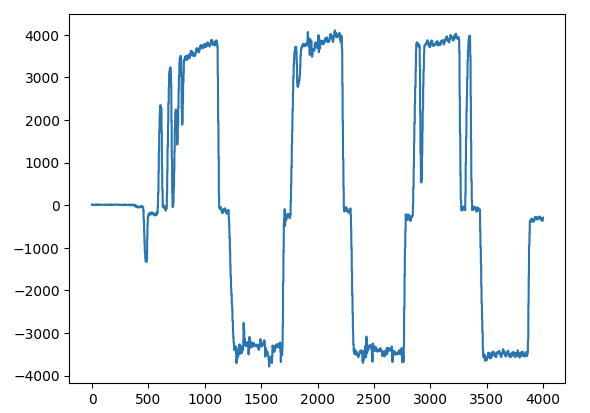
\includegraphics[width = \textwidth]{Figures/LapManual.png}
        \label{fig:LapsManual}
        \caption{Manuální řízení.}
    \end{subfigure}
    \captionsetup{justification=centering}
    \caption{Boční zrychlení během experimentů.}
    \label{fig:Laps}
\end{figure}

Implementace algoritmu prahování zajišťuje pro každý datový bod hodnotu úhlové
rychlosti z~gyroskopu na ose z. Pokud tato hodnota překročí prahovou hodnotu,
a~zároveň nebyla ještě zaznamenávaná zatáčka, algoritmus zaznamená časovou známku 
detekce jako počátek zatáčky. Zatáčka je stav, kdy gyroskop má nejvyšší hodnotu, 
což z~pohledu drahý je jedna ze dvou zatáček. Pokud hodnota úhlové rychlosti klesne 
pod prahovou hodnotu a~byla již zaznamenávaná zatáčka, znamená to, že byl detekován 
úplný kruh. Algoritmus poté zvýší počet detekovaných kol o~jednu. Tento proces se 
opakuje pro každý datový bod, čímž algoritmus umožňuje sledování a~počítání ujetých 
kol na základě úhlové rychlosti zaznamenané gyroskopem. 

Použitý algoritmus je ve výpisu:

\begin{lstlisting}[language = python, caption = Počet kol, label = lst:countLap]
threshold = 3000
half_lap_detected = False
lap_count = 0
laps = []
for data_point in data:
    if data_point.sensor.gyro.z >= threshold and not half_lap_detected:
        laps.append((lap_count, data_point.timestamp))
        half_lap_detected = True
    elif data_point.sensor.gyro.z <= -threshold and half_lap_detected:
        lap_count += 1
        half_lap_detected = False
\end{lstlisting}

Porovnání automatického se senzory i~bez senzoru a~manuálního řízení je v~tabulce 
\ref{tab:Comparison}. Čísla v~tabulce jsou počet tiků časovače za jedno kolo.
\begin{table}[!h]
    \centering
    \begin{tabular}{cccc}
        \hline
        \textbf{Řízení} & \textbf{1 Kolo} & \textbf{2 Kolo} & \textbf{3 Kolo} \\
        \hline
        Automatické se~senzory          & 921       & 906 & 932          \\
        Automatické bez senzoru & 982 & 953 & 963 \\
        Manuální 			  & 1178       & 1085 & 1161           \\
        \hline
    \end{tabular}
    \caption{Porovnání manuálního a~automatického řízení.}
    \label{tab:Comparison}
\end{table}

Na základě tabulky můžeme vyvodit závěr, že automatické řízení bez senzorů je 
rychlejší než manuální řízení, a~zároveň, že automatické řízení se senzory je 
nejrychlejší.

\endinput